
\chapter{Phase}

\section{Intro}
Intro stuff goes here.

\section{Resistors, Capacitors, and Inductors}

\begin{figure}[htbp]
\begin{center}
\begin{tabular}{ccc}
\begin{circuitikz}[line width=1pt]
\draw (0,0) node[left]{A} to[short,o-] ++(1.0,0) to[R,l=$R$] ++(0,+4.0) to[short, i<=$I$,-o] ++(-1.0,0) node[left]{B};
\draw (0,-1) node[]{$V_{AB} = IR$};
\end{circuitikz} &
\begin{circuitikz}[line width=1pt]
\draw (0,0) node[left]{A} to[short,o-] ++(1.0,0) to[C,l=$C$] ++(0,+4.0) to[short, i<=$I$,-o] ++(-1.0,0) node[left]{B};
\draw (1.7,2.4) node[left]{$Q$};
\draw (0,-1) node[]{$V_{AB} = \frac{Q}{C}$};
\end{circuitikz} &
\begin{circuitikz}[line width=1pt]
\draw (0,0) node[left]{A} to[short,o-] ++(1.0,0) to[L,l=$L$] ++(0,+4.0) to[short, i<=$I$,-o] ++(-1.0,0) node[left]{B};
\draw (0,-1) node[]{$V_{AB} = L \frac{dI}{dt}$};
\end{circuitikz} \\
(a) & (b) & (c) \\
\end{tabular}
\caption{The voltage across a (a) resistor, (b) capacitor, and (c) inductor.  The sign convention for all of these relationships implies that the component is being treated as a load, with current $I$ entering the positive terminal.  The charge $Q$ is the charge which builds up on the upper plate, while the lower plate will have charge $-Q$.}
\label{fig:rlc}
\end{center}
\end{figure}

We've already encountered our first two terminal electrical component, the resistor, which obeys Ohm's law.  When considering the sign of Ohm's law, one must remember that the definition implies that the resistor is being considered  as a load, as shown in Fig.~\ref{fig:rlc}a, with positive current directed into the positive terminal defining the voltage drop across the component.

A capacitor is a two terminal electrical component which stores energy in an electric field.  The electric field is the result of a build up of charge, positive on one terminal of the capacitor and negative on the other, which produces the electric field.  When considered as a load, with charge $Q$ on the upper terminal (and charge $-Q$ on the lower terminal) the voltage across a capacitor is:
\begin{displaymath}
V = \frac{Q}{C}
\end{displaymath}

An inductor is a two terminal electrical component which stores energy in a magnetic field when an electrical current passes through it.  Because of the property of self-inductance, an inductor tends to resist changes in current.  When considered as a load, the voltage across an inductor is:
\begin{displaymath}
V = L\frac{dI}{dt}
\end{displaymath}

While the capacitor and the inductor have the capability to store energy, none of these three components are capable of adding power to a circuit, and are therefore called passive components.

\section{Time dependence of a Capacitive Circuit}

\begin{figure}[htbp]
\begin{center}
\begin{circuitikz}[line width=1pt]
\draw (0,0) node[right]{A} to[short,o-*] coordinate(X) ++(-1.0,0) coordinate(X) to[C,l=$C$,i<=$I(t)$] ++(0,4.0) to[short,-o] ++(1.0,0) node[right]{B};
\draw (X) to[short,*-] ++ (-2.0,0) to[voltage source,bipoles/length=1.5cm,l=$V_0$] ++(0,+2.0)
to[cspst, bipoles/length=2.0cm] ++(0,2.0) to[resistor,l=$R$] ++(2.0,0);
\draw (-1.0,2.3) node[right]{$Q(t)$};
\end{circuitikz} 
\caption{Circuit for considering the behavior of a capacitor.}
\label{fig:rc}
\end{center}
\end{figure}

Consider the $RC$ circuit of Fig.~\ref{fig:rc} with the switch closed.  From KVL:
\begin{displaymath}
0 = V_0 - IR - \frac{Q}{C}
\end{displaymath}
or matching source voltage to load voltage:
\begin{displaymath}
V_0 = IR + \frac{Q}{C}
\end{displaymath}
The charge as a function of time $Q(t)$ therefore obeys the differential equation:
\begin{equation} \label{eqn:icap}
V_0 = \frac{dQ}{dt}R + \frac{Q(t)}{C}
\end{equation}
Our physical intuition leads us to try first for a steady-state solution of the form $Q(t) = Q_{\rm F}$ for some constant $Q_{\rm F}$, so that:
\begin{displaymath}
\frac{dQ}{dt} = 0
\end{displaymath}
and so Equation~\ref{eqn:icap} leads to:
\begin{displaymath}
Q_{\rm F} = C V_0.
\end{displaymath}
After enough time, the capacitor will charge to $CV_0$, the voltage across the capacitor will be equal to the applied voltage $V_0$, and so no current flow.  This is the steady-state behavior for this circuit.

However, imagine that at time $t=0$, the capacitor is initially uncharged with $Q=0$.  How will the circuit reach the steady-state?  Since the differential equation is linear, any solution to the homogenous version  (obtained by setting $V_0=0$):
\begin{equation} \label{eqn:hcap}
0 = \frac{dQ}{dt}R + \frac{Q(t)}{C}
\end{equation}
can be added to the steady-state solution to provide a solution to the non-homogenous version (with $V_0 \ne 0$).  Differential equations which relate the rate of change of a quantity to the quantity itself invariably lead to the exponential function, and we are led to try:
\begin{displaymath}
Q(t) = A \exp(B t)
\end{displaymath}
for constants $A$ and $B$.  Applying Equation~\ref{eqn:hcap} leads to:
\begin{eqnarray*}
0 &=& R B A \, \exp(B t)  + \frac{Q(t)}{C}\\
0 &=& \left( RB + \frac{1}{C}\right) Q(t)
\end{eqnarray*}
which will be true provided that:
\begin{displaymath}
B = -\frac{1}{RC}
\end{displaymath}
That is solutions of the form:
\begin{displaymath}
Q(t) = A \, \exp(- t/\tau)
\end{displaymath}
with $\tau = RC$ satisfy Equation~\ref{eqn:hcap} and can be added to the steady state solution to obtain:
\begin{displaymath}
Q(t) = CV_0 + A \, \exp(- t / \tau)
\end{displaymath}
which is the general solution to Equation~\ref{eqn:icap}.  (You can confirm this for yourself if this is the first time you have seen this approach used.)

For the specific case that $Q(0) = 0$, we conclude that $A = -CV_0$ and so:
\begin{displaymath}
Q(t) = CV_0 \left(1 - \exp(- t / \tau) \right)
\end{displaymath}
which describes a capacitor charging with a time constant $\tau = RC$ asymptotically approaching the steady-state $Q = CV_0$.  If follows that the voltage across the capacitor as a function of time is:
\begin{displaymath}
V(t) = \frac{Q(t)}{C} = V_0 \left(1 - \exp(- t / \tau) \right)
\end{displaymath}
while the current as a function of time is:
\begin{displaymath}
I(t) = \frac{dQ}{dt} = \frac{V_0}{R} \exp(- t / \tau) 
\end{displaymath}

The voltage and current as function of time for a charging capacitor is shown in Fig.~\ref{fig:vit_trans}
Notice that at $t=0$, we have simply $I = V_0/R$, as there is no voltage across the capacitor while $Q=0$.

\begin{figure}[htbp]
\begin{center}
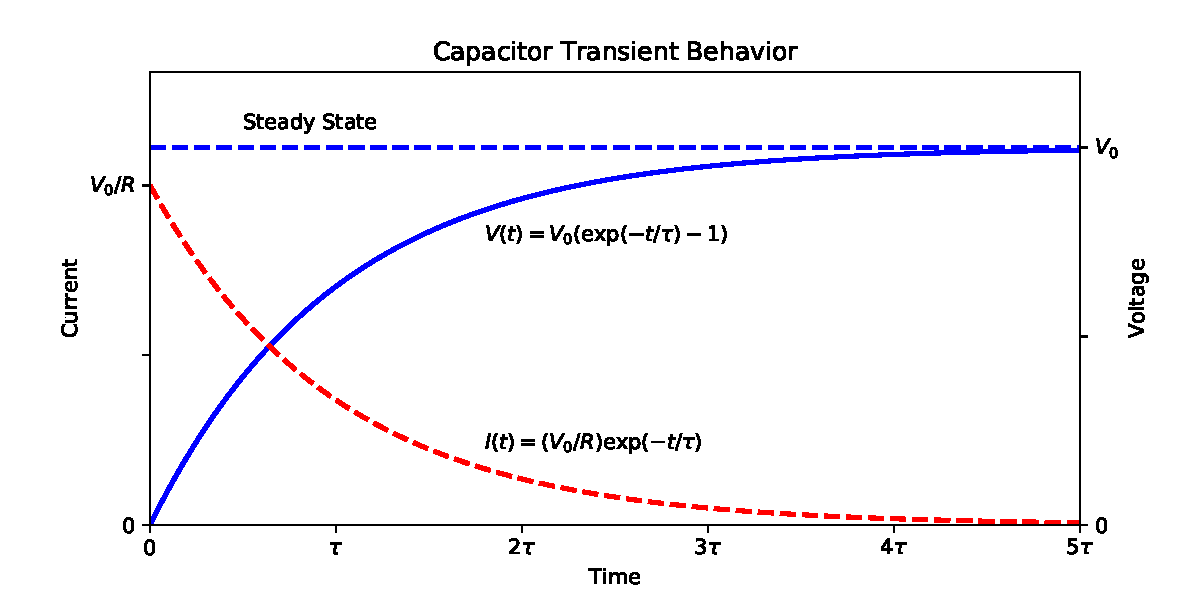
\includegraphics[height=0.3\textheight]{figs/transient_cap.pdf} \\
\caption{Current and voltage across a charging capacitor as a function of time.}
\label{fig:vit_trans}
\end{center}
\end{figure}

\section{Time dependence of an Inductive Circuit}

\begin{figure}[htbp]
\begin{center}
\begin{circuitikz}[line width=1pt]
\draw (0,0) node[right]{A} to[short,o-*] coordinate(X) ++(-1.0,0) coordinate(X) to[L,l=$L$,i<=$I$] ++(0,4.0) to[short,-o] ++(1.0,0) node[right]{B};
\draw (X) to[short,*-] ++ (-2.0,0) to[voltage source,bipoles/length=1.5cm,l=$V_0$] ++(0,+2.0)
to[cspst, bipoles/length=2.0cm] ++(0,2.0) to[resistor,l=$R$] ++(2.0,0);
\end{circuitikz} 
\caption{\label{fig:rl} Circuit for considering the behavior of an inductor.}
\end{center}
\end{figure}

Consider the $RL$ circuit of Fig.~\ref{fig:rl} with the switch closed.  From KVL:
\begin{displaymath}
0 = V_0 - IR - L\frac{dI}{dt}
\end{displaymath}
or matching source voltage to load voltage:
\begin{displaymath}
V_0 = IR + L\frac{dI}{dt}
\end{displaymath}
The current as a function of time $I(t)$ therefore obeys the differential equation:
\begin{equation} 
V_0 = R I(t) + L \frac{dI}{dt}
\end{equation}
It is left as an exercise to show that the steady-state solution is the constant current:
\begin{equation} \label{eqn:inductorss}
I = V_0 / R
\end{equation}
and the general solution is 
\begin{equation} \label{eqn:inductorgen}
I(t) = (V_0 / R) + A \, \exp(-t/\tau) 
\end{equation}
with $\tau = L / R$.

For the specific case that $I(0) = 0$, we conclude that $A = -V/R$ and so:
\begin{displaymath}
I(t) = (V_0/R) \, (1 - \exp(-t / \tau)).
\end{displaymath}

% TODO:  show V(t)

\section{Alternating Current}

% TODO:  needs a figure

 We've seen now that voltages can be a function of time $V(t)$.    If the steady-state voltage levels in a circuit are constant with time, it is referred to as a direct current (DC) circuit, because the currents that result tend to flow in the same direction.   A circuit with a time-dependence which averages to zero by oscillating back and forth is referred to as an alternating current (AC).   If the voltage is changing with time, but does not average to zero, the signal is a mixture of AC and DC.  The DC contribution is the average value, and the AC component is what remains when this DC component is removed.  We will use a convention that lower-case variables, such as $v$ and $i$ refer to AC quantities, and upper case variables, such as $V$ and $I$ refer to DC quantities.  Transients responses, which are often ignored in AC and DC circuit analysis, will remain as time-dependent upper case variables, such as $V(t)$ and $I(t)$.
   
Of particular importance, is a sinusoidal voltage of the form:
 \begin{displaymath}
 v(t) = v_{\rm p} \cos(\omega t + \phi).
 \end{displaymath}
 The parameter $v_p$ in this equation is called the peak AC voltage.  The parameter $\omega$ is the angular frequency, related to the frequency $f$ by $\omega = 2 \pi f$.  The parameter $\phi$ determines the phase of the voltage.

Other common measurements of the AC voltage level are the peak-to-peak AC voltage, which for a pure sine wave is:
\begin{displaymath}
v_{\rm pp} = 2 v_{\rm p}.
\end{displaymath}
And the root-mean-square (RMS) average AC voltage:
\begin{displaymath}
v_{\rm rms} = \sqrt{\langle v^2(t) \rangle}
\end{displaymath}
where $\langle f(t) \rangle$ denotes the time average:
\begin{displaymath}
\langle f(t) \rangle \equiv \frac{1}{T}\int_{-T/2}^{T/2} f(t)
\end{displaymath}
It is left as an exercise to show that for a pure sine wave:
\begin{displaymath}
v_{\rm rms} = v_{\rm p} / \sqrt{2}
\end{displaymath}
When left unspecified, an AC voltage usually refers to an RMS voltage.  So when we refer to a $120~\rm V$ household outlet, we mean specifically a $120~\rm V$~(AC) RMS voltage.  

Understanding the response of circuits to AC voltages is of paramount importance.  This is not just because our power arrives as an AC voltage.  Much of modern electronics, both at home and in the lab, is used for signal processing of time dependent signals encoded as $V(t)$.  Fourier's Theorem informs us that any time-dependent signal can be interpreted as a sum of sine and cosine functions of different frequencies.  So if we can understand the response of our circuit to DC plus AC sine waves of any frequency, we know everything there is to know about the circuit.

\section{Passive Components and Alternating Current}

\begin{figure}[htbp]
\begin{center}
\begin{circuitikz}[line width=1pt]
\draw (0,0) coordinate(X) to[sinusoidal voltage source,bipoles/length=1.5cm] ++(0,+2.0) 
to [short,i=$i$] ++(1.5,0) to[R,l_=$R$] ++(0,-2.0) to[short] ++(-1.5,0);
\draw (X) node[ground,yscale=2.0]{};
\draw (0.0,1.7) node[left]{$v(t)$};
\end{circuitikz} 
\caption{An AC voltage source applied to a resistor.}
\label{fig:acr}
\end{center}
\end{figure}

We are now ready to consider what happens to resistors, capacitors, and inductors when an AC voltage is applied across them.  We'll start with the easiest case, the resistor, and the circuit illustrated in Fig.~\ref{fig:acr}.  We've introduced a new symbol, the AC voltage source.  We'll adopt the convention that the positive terminal is always at the top.  We'll also reference the negative terminal to ground, because the function generator you use in lab is referenced to ground.  To reinforce the convention that the positive terminal is at the top, that is where we will label the time dependent voltage provided, which we will take in most cases as:
\begin{displaymath}
v(t) = v_{\rm p} \cos(\omega t).
\end{displaymath}
In the case of the resistor, Ohm's law informs us immediately that:
\begin{displaymath}
i(t) = v(t) / R = (1/R) \, v_{\rm p} \cos(\omega t)
\end{displaymath}
If we are only concerned with the RMS current and voltage, we find:
\begin{displaymath}
v_{\rm rms}/i_{\rm rms} = R 
\end{displaymath}
Ohm's law is alive and well for AC circuits!

\begin{figure}[htbp]
\begin{center}
\begin{circuitikz}[line width=1pt]
\draw (0,0) coordinate(X) to[sinusoidal voltage source,bipoles/length=1.5cm] ++(0,+2.0) 
to [short,i=$i$] ++(1.5,0) to[C,l_=$C$] ++(0,-2.0) to[short] ++(-1.5,0);
\draw (X) node[ground,yscale=2.0]{};
\draw (0.0,1.7) node[left]{$v(t)$};
\end{circuitikz} 
\caption{An AC voltage source applied to a capacitor.}
\label{fig:acr}
\end{center}
\end{figure}

The capacitance relates the voltage to the charge on the capacitor:
\begin{displaymath}
q(t)  = C v(t)
\end{displaymath}
and so taking the derivative with respect to time:
\begin{displaymath}
i = \frac{dq}{dt} = C \frac{dv}{dt}
\end{displaymath}
So in this case, with $v(t) = v_p \cos(\omega t)$
\begin{eqnarray*}
i &=& C (-\omega v_p \sin(\omega t))\\
 &=& (\omega C) v_p \cos \left( \omega t + \frac{\pi}{2} \right) \\
\end{eqnarray*}
The RMS values are related by:
\begin{displaymath}
v_{\rm rms}/i_{\rm rms} = \frac{1}{\omega C}
\end{displaymath}
but the phase of the voltage relative to the current is $\Delta \phi = -\pi/2$ (due to the $+\pi/2$ term in the current.)

\begin{figure}[htbp]
\begin{center}
\begin{circuitikz}[line width=1pt]
\draw (0,0) coordinate(X) to[sinusoidal voltage source,bipoles/length=1.5cm] ++(0,+2.0) 
to [short,i=$i$] ++(1.5,0) to[L,l_=$L$] ++(0,-2.0) to[short] ++(-1.5,0);
\draw (X) node[ground,yscale=2.0]{};
\draw (0.0,1.7) node[left]{$v(t)$};
\end{circuitikz} 
\caption{An AC voltage source applied to a inductor.}
\label{fig:acr}
\end{center}
\end{figure}

The inductance relates the voltage to the rate of change of the current:
\begin{displaymath}
\frac{di}{dt}  =\frac{1}{L} v(t)
\end{displaymath}
and so integrating with respect to time:
\begin{displaymath}
i = \frac{1}{L} \int dt \; v(t) 
\end{displaymath}
So in this case, with $v(t) = v_p \cos(\omega t)$
\begin{eqnarray*}
i &=& \frac{1}{L}  \int dt \; v_p \cos(\omega t)\\ 
&=& \frac{1}{L} \left( \frac{v_p}{\omega} \sin(\omega t) \right) + I_0\\
&=& \frac{1}{\omega L} \cos \left( \omega t - \frac{\pi}{2} \right)  + I_0\\
\end{eqnarray*}
The constant of integration $I_0$ is a constant direct current.  Indeed, with no resistance in this idealized circuit, a DC current could flow indefinitely, with no DC voltage drop anywhere in the circuit.  Of course, in a real circuit with resistance, such a current would quickly disappear.  We'll simply assume $I_0=0$ for our purpose of understanding the AC response, and so:
\begin{eqnarray*}
i &=& \frac{1}{\omega L} \cos \left( \omega t - \frac{\pi}{2} \right)\\
\end{eqnarray*}
The RMS values are related by:
\begin{displaymath}
v_{\rm rms}/i_{\rm rms} = \omega L
\end{displaymath}
but the phase of the voltage relative to the current is $\Delta \phi = \pi/2$ (due to the $-\pi/2$ term in the current.)

\begin{figure}[htbp]
\begin{center}
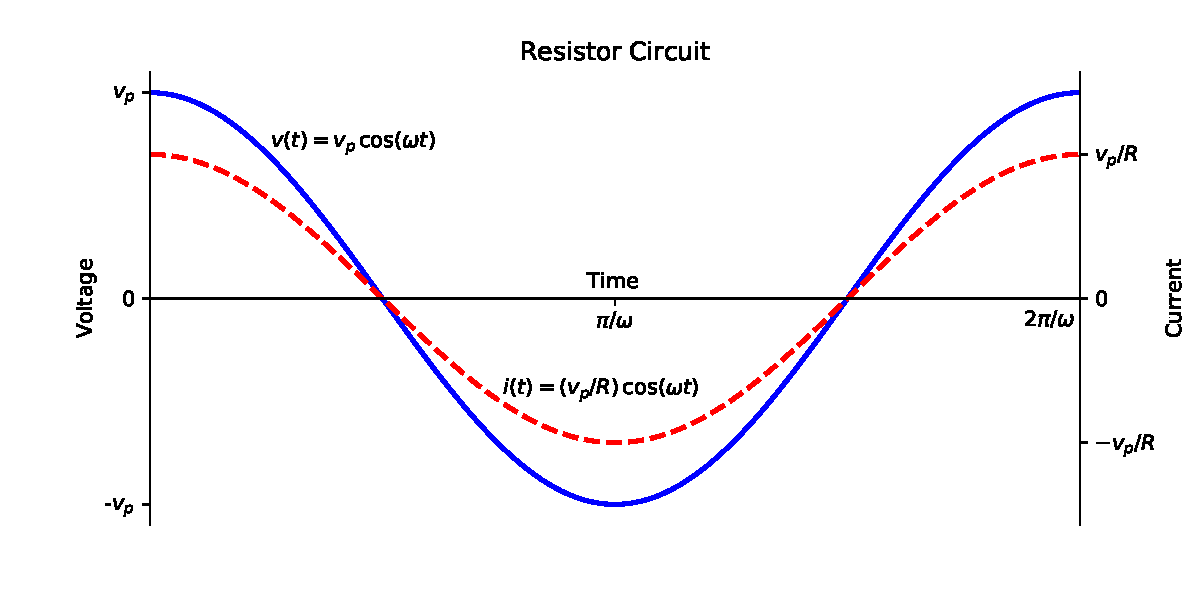
\includegraphics[height=0.3\textheight]{figs/vit_res.pdf} \\
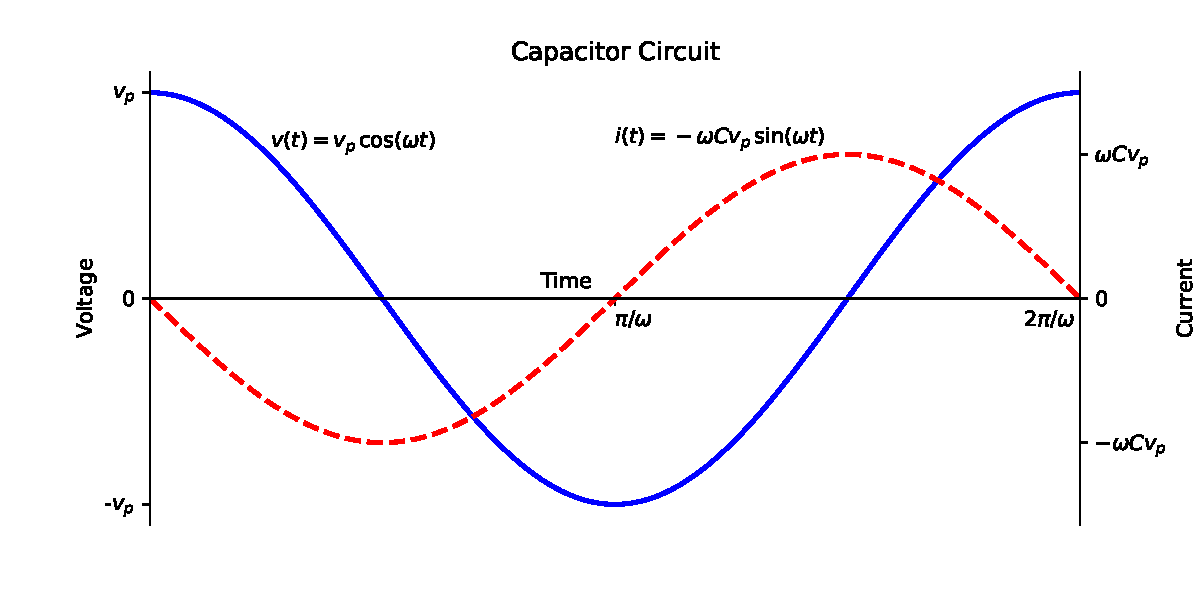
\includegraphics[height=0.3\textheight]{figs/vit_cap.pdf} \\
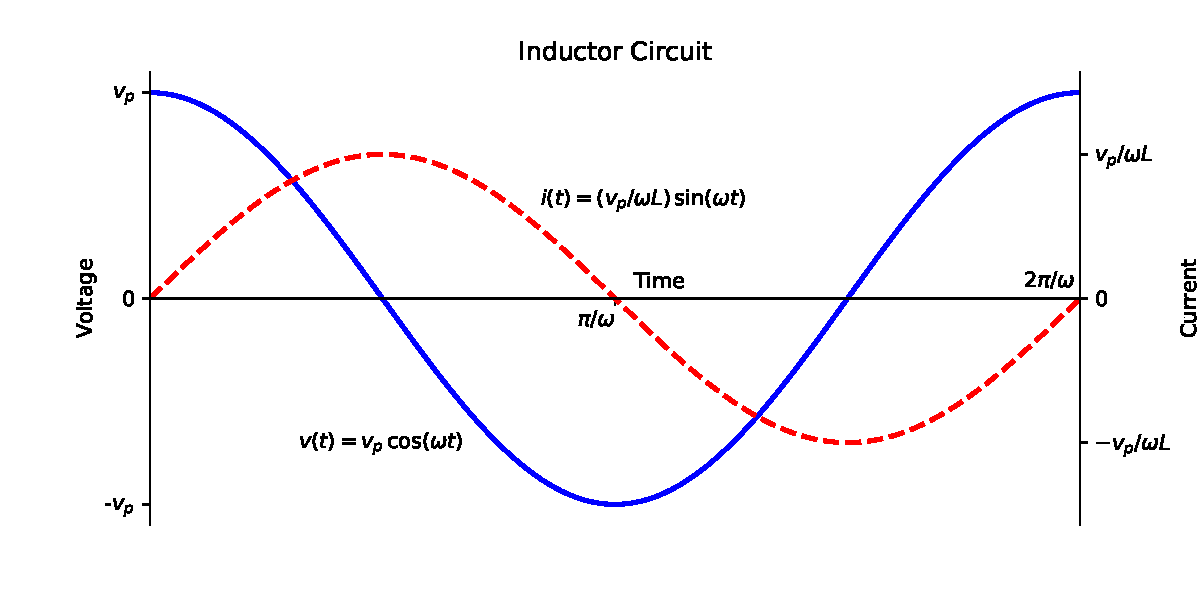
\includegraphics[height=0.3\textheight]{figs/vit_ind.pdf} \\
\caption{ Time dependence of AC voltage and current in a resistor, capacitor, or inductor.}
\label{fig:vit}
\end{center}
\end{figure}



\begin{table}
\caption{Summary or relationship between current and voltage for AC signals.}
\label{tbl:rmsimp}
\begin{center}
\begin{tabular}{lrr}
component & $v_{\rm rms} / i_{\rm rms} $ & $\Delta \phi$ \\
\hline
\\
resistor ($R$) & $R$ & $0$ \\
\\
capacitor ($C$) & $\displaystyle \frac{1}{\omega C}$ & $\displaystyle -\frac{\pi}{2}$ \\
\\
inductor ($L$) & $\omega L$ & $\displaystyle +\frac{\pi}{2}$ \\
\\
\end{tabular}
\end{center}
\end{table}

The present situation is summarized in Table~\ref{tbl:rmsimp} and Fig.~\ref{fig:vit}, and it is tempting to think we are finished.  After all, we've found an Ohm's Law like relationship between $v_{\rm rms}$ and $i_{\rm rms}$ for capacitors and inductors, so shouldn't we able to analyze AC circuits just like DC circuits?  The problem is that we do not yet have an equivalent for Kirchoff's Laws.  DC voltages and currents simply add, but now our voltages have a phase, so we can't, for instance, simply add RMS voltages.  Faced with a more complicated circuit, we could derive a new, more complicated differential equation, and solve that.  Fortunately, there's an easier way!

\section{Phasors}

\begin{figure}[htbp]
\begin{center}
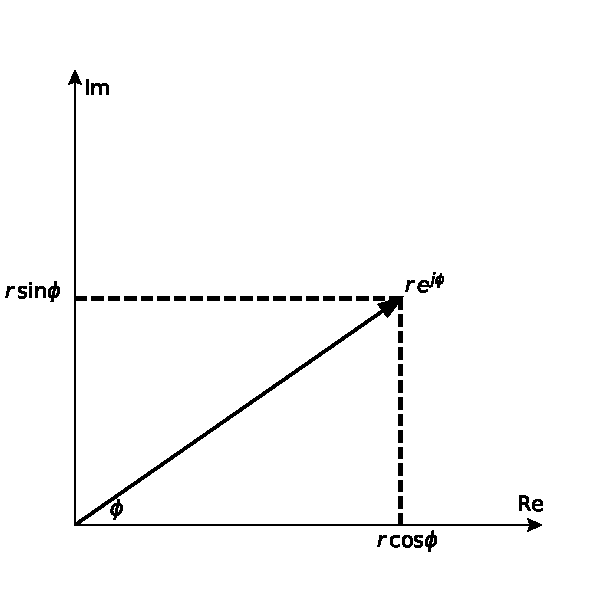
\includegraphics[height=0.3\textheight]{figs/complex.pdf} \\
\caption{ The geometry of the complex plane.}
\label{fig:complex}
\end{center}
\end{figure}

Recall Euler's Formula, which Feynman called ``our jewel'':
\begin{displaymath}
e^{j\phi} = \cos \phi + j \sin \phi 
\end{displaymath}
where we will use $j$ as the unit imaginary number, to avoid confusion with the AC current $i$.  This result has a beautiful geometric interpretation that allows us to consider the real and imaginary parts of a complex number as two components of a vector which has a magnitude and phase.  In particular, we can relate the cosine function to the real part of an imaginary number:
\begin{displaymath}
r \cos \phi = \Re \{ r e^{j\phi} \}. 
\end{displaymath}
We can therefore consider any AC signal:
\begin{displaymath}
v(t) = v_{\rm p} \cos ( \omega t + \phi)
\end{displaymath}
to be the real part of a time-dependent complex number:
\begin{displaymath}
v(t) = \Re \{ v_{\rm p} \exp ( j (\omega t + \phi))\}.
\end{displaymath}
We can rearrange this complex number as:
\begin{eqnarray*}
v(t) &=& \Re \{ v_{\rm p} e^{j\phi} \cdot e^{j \omega t} \} \\
&=& \Re \{ \tilde{v} \cdot e^{j \omega t} \} \\
\end{eqnarray*}
where we have defined the quantity:
\begin{equation}
\tilde{v} \equiv v_{\rm p} e^{j \phi}
\label{eqn:phasor}
\end{equation}

which we call a phase vector or simply phasor.  The phasor is a complex number that contains the magnitude and phase information for the particular AC signal we are considering.  It is simply a complex number, with no time dependence.  The time-dependent part of the entire expression comes from the term $e^{j \omega t}$, and is the same for every AC signal of frequency $\omega$.  Once we have specified the frequency of an AC circuit, there is a one-to-one corresponds with time dependent functions like v(t), and the phasor.  The phasor for an AC signal $v(t) = v_{\rm p} cos(\omega t + \phi)$ is given by the definition in Equation~\ref{eqn:phasor}.  To obtain the time-dependent signal from a phasor we simply calculate:
\begin{equation}
v(t) = \Re \{ \tilde{v} e^{j \omega t} \}
\end{equation}

\section{Impedance}

\begin{figure}[htbp]
\begin{center}
\begin{tabular}{ccc}
\begin{circuitikz}[line width=1pt]
\draw (0,0) coordinate(X) to[sinusoidal voltage source,bipoles/length=1.5cm] ++(0,+2.0) 
to [short,i=$\tilde{i}$] ++(1.5,0) to[R,l_=$R$] ++(0,-2.0) to[short] ++(-1.5,0);
\draw (X) node[ground,yscale=2.0]{};
\draw (0.0,1.7) node[left]{$\tilde{v}$};
\end{circuitikz} &
\begin{circuitikz}[line width=1pt]
\draw (0,0) coordinate(X) to[sinusoidal voltage source,bipoles/length=1.5cm] ++(0,+2.0) 
to [short,i=$\tilde{i}$] ++(1.5,0) to[C,l_=$C$] ++(0,-2.0) to[short] ++(-1.5,0);
\draw (X) node[ground,yscale=2.0]{};
\draw (0.0,1.7) node[left]{$\tilde{v}$};
\end{circuitikz} &
\begin{circuitikz}[line width=1pt]
\draw (0,0) coordinate(X) to[sinusoidal voltage source,bipoles/length=1.5cm] ++(0,+2.0) 
to [short,i=$\tilde{i}$] ++(1.5,0) to[L,l_=$L$] ++(0,-2.0) to[short] ++(-1.5,0);
\draw (X) node[ground,yscale=2.0]{};
\draw (0.0,1.7) node[left]{$\tilde{v}$};
\end{circuitikz} \\
(a) & (b) & (c) \\
\end{tabular}
\caption{An AC voltage source applied to (a) a resistor, (b) a capacitor, and (c) an inductor.}
\label{fig:aclcr}
\end{center}
\end{figure}

For a resistor driven by a sinusoidal voltage source as in Fig.~\ref{fig:aclcr}a, Ohm's law states that:
\begin{displaymath}
i(t) = v(t) / R 
\end{displaymath}
If we write v(t) in terms of its associated phasor $\tilde{v}$:
\begin{eqnarray*}
i(t) &=& \frac{\Re \{ \tilde{v} \; e^{j \omega t}\}}{R} \\
&=& \Re \left\{ \frac{\tilde{v}}{R} \; e^{j \omega t} \right\} \\
\end{eqnarray*}
we can see that $i(t)$ is itself associated with the phasor:
\begin{displaymath}
\tilde{i} = \frac{\tilde{v}}{R}
\end{displaymath}
and so there is an Ohm's Law relationship between the phasors:
\begin{displaymath}
\tilde{v} = R \; \tilde{i}
\end{displaymath}

For a capacitor driven by a sinusoidal voltage source as in Fig.~\ref{fig:aclcr}b, we showed above that the current is related to the derivative of the voltage:
\begin{displaymath}
i(t) = C \, \frac{dv}{dt}
\end{displaymath}
If we write v(t) in terms of its associated phasor $\tilde{v}$:
\begin{eqnarray*}
i(t) &=& C \, \frac{d}{dt} \, \Re \{ \tilde{v} \; e^{j \omega t}\} \\
&=& \Re \left\{ \tilde{v} C \frac{d}{dt} \; e^{j \omega t} \right\} \\
&=& \Re \left\{ \tilde{v} j \omega C \; e^{j \omega t} \right\} \\
\end{eqnarray*}
where in the last step we have used the fact that:
\begin{displaymath}
\frac{d}{dt} e^{\alpha t} = \alpha e^{\alpha t}.
\end{displaymath}
From:
\begin{eqnarray*}
i(t) &=& \Re \left\{ \tilde{v} j \omega C \; e^{j \omega t} \right\} \\
\end{eqnarray*}
we can see that $i(t)$ is associated with the phasor:
\begin{displaymath}
\tilde{i} = j \omega C \tilde{v}
\end{displaymath}
which we can think of as Ohm's Law for a capacitor:
\begin{displaymath}
\tilde{v} = \frac{1}{j \omega C} \tilde{i}
\end{displaymath}
It's worth taking a moment to marvel over what we have accomplished here:  we replaced the differential equation describing the relations between $v(t)$ and $i(t)$ with mere multiplication of a phasor by a complex number.  We can analyze circuits simply according to the phasors, and convert our answer to time dependent signals whenever needed.  We already knew that the magnitude of the voltage and current were simply related.  By using phasors, one complex number describes the change in magnitude and the change in phase.

Now let's turn to the inductor, driven by a sinusoidal voltage source as in Fig.~\ref{fig:aclcr}c, for which we already determined that current is related to the integral of the voltage:
\begin{displaymath}
i = \frac{1}{L} \int dt \; v(t) 
\end{displaymath}
It is left as an exercise to show that the phasors for current and voltage are related by:
\begin{displaymath}
\tilde{v} = j \omega L \tilde{i}.
\end{displaymath}

\begin{table}
\caption{Impedances of passive-components}
\label{tbl:impedance}
\begin{center}
\begin{tabular}{ccc}
Component & Impedance & $\Delta \phi$ \\
\hline
\\
$R$ & $R$ & 0 \\
\\
$C$ & $\displaystyle \frac{1}{j \omega C}$ & $\displaystyle -\frac{\pi}{2}$ \\
\\
$L$ & $j \omega L$ & $\displaystyle +\frac{\pi}{2}$ \\

\end{tabular}
\end{center}
\end{table}

We've now shown that for all three of our passive components ($R$, $C$, and $L$) the phasor for voltage is simply the product of the phasor for the current times a complex number, which we call the impedance, $Z$.  We call the imaginary part of the impedance the reactance $X$, and the real part the resistance:
\begin{eqnarray*}
({\rm impedance}) &=& ({\rm resistance}) + j ({\rm reactance} ) \\
Z &=& R + j X \\
\end{eqnarray*}
These results are summarized in Table~\ref{tbl:impedance}.  

Kirchhoff's Voltage Laws and Kirchhoff's Current Law continue to hold for the time dependent voltages and currents, but they apply equally to the (constant valued) complex phasors.  A new Ohm's Law, which applies to all passive components states that:
\begin{displaymath}
\tilde{v} = Z \tilde{i}
\end{displaymath}
All of our previous results therefore apply with resistance replaced by impedance.  In particular, the impedance of components in series adds linearly:
\begin{equation} \label{eqn:zseries}
Z_{\rm eq} = \sum_i Z_i. 
\end{equation}
whereas for components in parallel:
\begin{equation} \label{eqn:zseries}
\frac{1}{Z_{\rm eq}} = \sum_i \frac{1}{Z_i}. 
\end{equation}




\section{Passive Filters}

\begin{figure}[htbp]
\begin{center}
\begin{tabular}{cc}
\begin{circuitikz}[line width=1pt]
\draw (0,0) node[ground,yscale=2.0]{} to[sinusoidal voltage source,bipoles/length=1.5cm] ++(0,+4.0) 
to [short,i=$\tilde{i}$] ++(1.5,0) to[R,l_=$R$] ++(0,-2.0) coordinate(B)
to[C,l_=$C$] ++(0,-2.0) coordinate(A) to[short] ++(-1.5,0);
\draw (0.0,2.75) node[left]{$\tilde{v}_{\rm in}$};
\draw (B) to[short,*-o] ++(1.5,0) node[right]{$\tilde{v}_{\rm out}$};
\end{circuitikz} &
\begin{circuitikz}[line width=1pt]
\draw (0,0) node[ground,yscale=2.0]{} to[sinusoidal voltage source,bipoles/length=1.5cm] ++(0,+4.0) 
to [short,i=$\tilde{i}$] ++(1.5,0) to[C,l_=$C$] ++(0,-2.0) coordinate(B)
to[R,l_=$R$] ++(0,-2.0) coordinate(A) to[short] ++(-1.5,0);
\draw (0.0,2.75) node[left]{$\tilde{v}_{\rm in}$};
\draw (B) to[short,*-o] ++(1.5,0) node[right]{$\tilde{v}_{\rm out}$};
\end{circuitikz} \\
(a) & (b) \\
\end{tabular}
\caption{Passive $RC$ (a) low-pass, and (b) high-pass filters.  Note that $\tilde{v}_{\rm in}$ and $\tilde{v}_{\rm out}$ are phasors corresponding to AC voltages referenced to ground.}
\label{fig:rcfilters}
\end{center}
\end{figure}

Consider the low-pass filter of Fig.~\ref{fig:rcfilters}a.   The output voltage $v_{\rm out}$ is simply the output of a voltage divider, but with the complex impedance taking the place of the resistance:
\begin{displaymath}
\tilde{v}_{\rm out} = \tilde{v}_{\rm in} \frac{Z_C}{Z_R + Z_C}
\end{displaymath}
And inserting the impedance of each device in terms of $R$ and $C$:
\begin{eqnarray*}
\tilde{v}_{\rm out} &=& \tilde{v}_{\rm in} \, \frac{\frac{1}{j \omega C}}{R + \frac{1}{j \omega C}}\\
&=& \tilde{v}_{\rm in} \, \frac{1}{1 + j \omega/\omega_0}\\
\end{eqnarray*}
Where we have defined the corner angular frequency: 
\begin{equation*}
\omega_0 = \frac{1}{RC}
\end{equation*}  
with corresponding corner frequency:
\begin{equation*}
f_0  \equiv \frac{\omega_0}{2\pi} = \frac{1}{2 \pi RC}.
\end{equation*}  
\begin{figure}[htbp]
\begin{center}
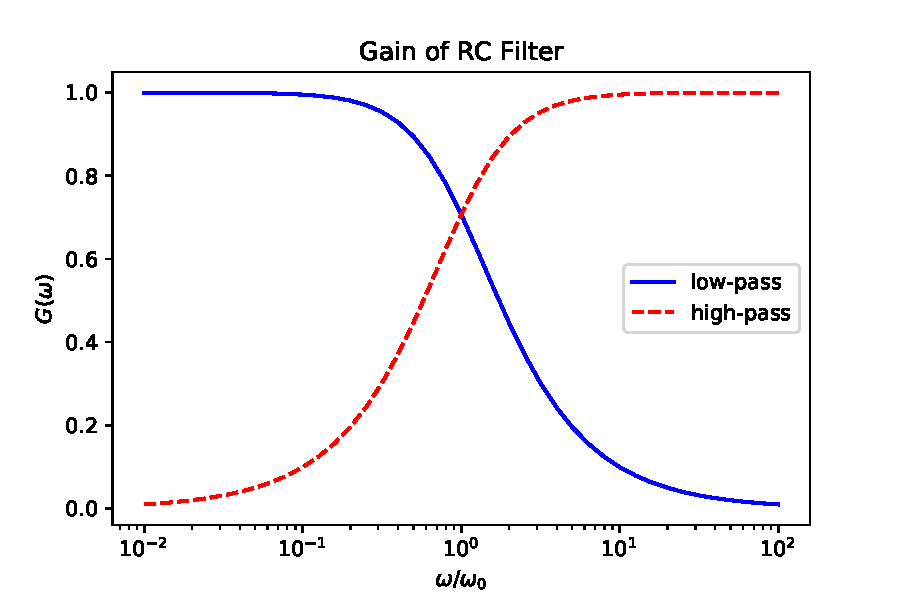
\includegraphics[height=0.3\textheight]{figs/rcgain.pdf} \\
\caption{ The gain of an RC filter.}
\label{fig:rcgain}
\end{center}
\end{figure}
We are particularly interested in the ratio of the output phasor to the input phasor, which defines the complex valued transfer function for the circuit $H(\omega)$:
\begin{equation*}
H(\omega) \equiv \frac{\tilde{v}_{\rm out}}{\tilde{v}_{\rm in}} = \frac{1}{1 + j \omega/\omega_0}\\
\end{equation*}
Our primary concern is generally the ratio of the amplitude of the output voltage to the amplitude of the input voltage, without concern for phase, which we call the gain $G(\omega)$:
\begin{equation*}
G(\omega) \equiv \frac{|\tilde{v}_{\rm out}|}{|\tilde{v}_{\rm in}|} = |H(\omega)| 
\end{equation*}
which is in this case:
\begin{eqnarray*}
G(\omega) &=& |H| = \frac{1}{|1 - j \omega/\omega_0 |}\\
&=& \frac{1}{\sqrt{1+\omega^2/\omega_0^2}}
\end{eqnarray*}
Notice that the gain is a positive real value that depends on the angular frequency $\omega$.
For the filter discussed here, at $\omega=0$, we see that $G=1$, while for $\omega \to \infty$, $G \to 0$.
At the corner frequency $\omega = \omega_0$, we see that $G = 1/\sqrt{2}$.
The function is plotted across five orders of magnitude in Fig.~\ref{fig:rcgain}.
We can see that below the corner frequency, the gain is everywhere nearly one, while above the corner frequency, the gain falls to zero.  Low-pass filters attenuate frequencies below the corner frequency while passing frequencies below the corner frequency unchanged.

It is left as an exercise to show that for the high-pass filter, with the roles of $R$ and $C$ interchanged, the transfer function is:
\begin{equation*}
H(\omega) \equiv \frac{\tilde{v}_{\rm out}}{\tilde{v}_{\rm in}} = \frac{1}{1 - j \omega_0/\omega}\\
\end{equation*}
with the corner angular frequency $\omega_0$ defined as before.  The gain is therefore:
\begin{equation*}
G(\omega) = \frac{1}{\sqrt{1+\omega_0^2/\omega^2}}
\end{equation*}
As shown in Fig.~\ref{fig:rcgain} the response of the high-pass filter is complementary to the low-pass filter:  the high-pass filter tends to reject signals with frequencies below the corner frequency while leaving signals with frequencies above the corner frequency unchanged.

\section{Decibels}

The decibel is an often confusing, yet widely used, system of measurement used to express the ratio of one value to another on a logarithmic scale.  Decibels were originally used to describe relative power in telecommunications systems, where the definition is:
\begin{equation}
dB = 10 \, \log_{10}(P_1 / P_0)
\end{equation}
where $P_1$ is the power we are describing relative to the power $P_0$.  In many system there is a quadratic relation between the power and another quantity, which is called a root-power quantity.
For instance, the power in a resistor is $P=V^2/R$.  When using a root-power quantity such as $V$, the definition of a dB is adjusted by a factor of two:
xo\begin{equation}
dB = 20 \, \log_{10}(V_1 / V_0)
\end{equation}
This allows us to refer to e.g. the $X$ dB point in a way that is independent of whether we refer to power or amplitude, an advantage of dubious value.

Things tend to get a bit more confusing when we move from using decibels to describe a ratio to describing a single quantity.  In this case, the reference value is added to the unit, e.g. dBV is decibel calculated with respect to a one Volt reference.   The special case of measuring power in milliWatts is given the unit dBm.  It is basically a nightmare of implicit definitions as a work-around for the inconvenient fact that the log function insists on a dimensionless quantity.

If you pick a nice sunny day, and linger outside Kemper hall long enough, you are all but guaranteed to hear someone mention ``the three dB point".   This benchmark point result from the unhappy\footnote{for those of that wish dB did not exist.} coincidence that:
\begin{equation*}
10 \log_{10} 2 = 3.01
\end{equation*}
In an $RC$ filter at the corner frequency with $\omega = \omega_0$, the voltage gain is $1/\sqrt{2}$ and the power gain is $1/2$, so the gain in dB is nearly -3.  For an RC circuit, the corner frequency is the ``negative three dB point.''

Undoubtably one reason the dB persists as a unit is that knowing the negative three dB point and then the easily calculated powers of 10 allows one to estimate the response of a system across a wide range:
\begin{eqnarray*}
20 \log_{10} \frac{1}{\sqrt{2}} &\sim& -3~\rm dB\\
20 \log_{10} \frac{1}{10} &=& -20~\rm dB\\
20 \log_{10} \frac{1}{100} &=& -40~\rm dB\\
\end{eqnarray*}
See Fig.~\ref{fig:rcbode}.

\section{Phase Change in Passive Filters}

So far we've considered only the effect of an $RC$ filter on the magnitude of the voltage.  We've yet to consider the phase.  This phase information is contained in complex valued transfer function:
\begin{displaymath}
H = \frac{\tilde{v}_{\rm out}}{\tilde{v}_{\rm in}} 
\end{displaymath}
The change in phase of the output relative to input is simply the polar coordinate $\phi$ of the complex number $H$:
\begin{displaymath}
\phi(H) = \tan^{-1}\left( \frac{\Im{H}}{\Re{H}}\right)
\end{displaymath}
Which in the case of a low-pass filter, results in the phase change:
\begin{displaymath}
\phi = -\tan^{-1} \left( \frac{\omega}{\omega_0}\right)
\end{displaymath}
and for the high-pass filter:
\begin{displaymath}
\phi = \tan^{-1} \left( \frac{\omega_0}{\omega}\right)
\end{displaymath}
as illustrated in Fig.~\ref{fig:rcbode}.  When considering phase changes, it's useful to consider the following benchmarks:
\begin{eqnarray*}
\tan^{-1}(1)  &=& \frac{\pi}{4} = 45^\circ\\
\tan^{-1}(0.1)  &=& 6^\circ\\
\tan^{-1}(10.0)  &=& 90 - 6^\circ\\
\end{eqnarray*}
So we can see that the phase change at the corner frequency is $45^\circ$ and is within $6^\circ$ of the asymptotic value after 1 order of magnitude in frequency.

\begin{figure}[htbp]
\begin{center}
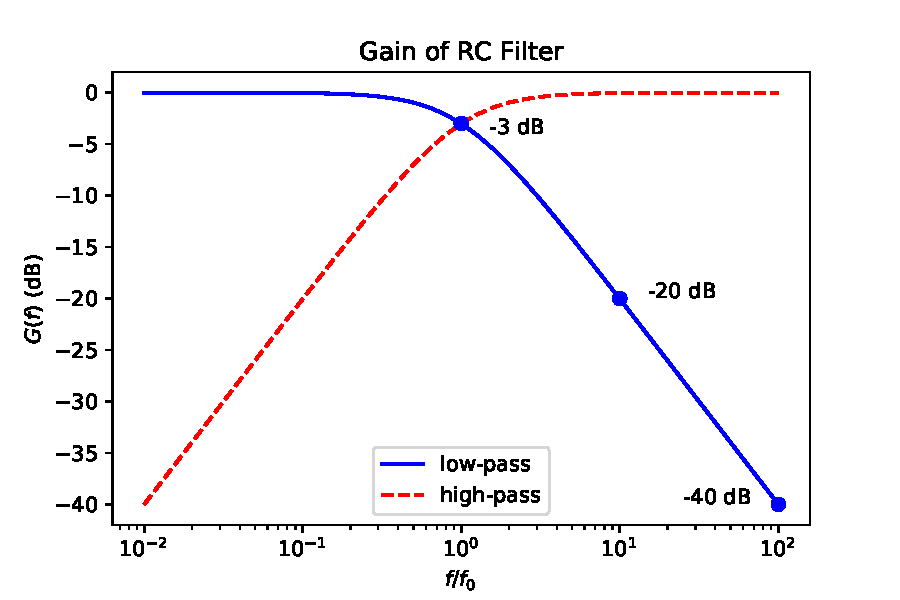
\includegraphics[height=0.3\textheight]{figs/rcgaindb.pdf} \\
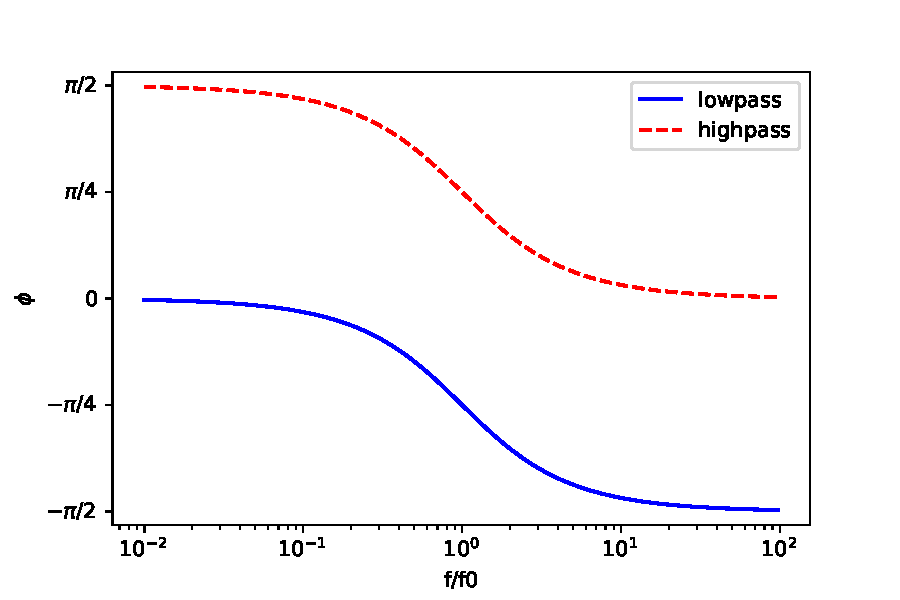
\includegraphics[height=0.3\textheight]{figs/rcphase.pdf} \\
\caption{ The upper plot shows the gain in decibels of an RC filter as a function of frequency, while the lower plot shows the corresponding phase shifts.  Together, these are referred to as the Bode plots for the filter (pronounced ``boh-dee".)}
\label{fig:rcbode}
\end{center}
\end{figure}


\section{Band Pass Filters}


\begin{figure}[htbp]
\begin{center}
\begin{circuitikz}[line width=1pt]
\draw (0,0) node[ground,yscale=2.0]{} to[sinusoidal voltage source,bipoles/length=1.5cm] ++(0,+4.0) 
to [short,i=$\tilde{i}$] ++(1.5,0) to[R,l_=$R$] ++(0,-1.5) coordinate(B) to[short]++(0,-0.5) coordinate(C) to[short]++(-0.5,0) coordinate(D) to[short]++(1,0) coordinate(E);
\draw (E) to [C,l_=$C$] ++(0,-1.5) coordinate(A) to [short]++(-0.5,0)  to [short]++(0,-0.5) to [short]++(-1.5,0);
\draw(D) to [L,l_=$L$]++(0,-1.5) coordinate(A) to [short]++(0.5,0);
%to[C,l_=$C$] ++(0,-2.0) coordinate(A) to[short] ++(-1.5,0);
%\draw (X) to[C,-*,l=$C_1$] ++(0,-3.0)  to[short,-*] ++(-2.0,0) node[ground,yscale=2.0]{};
\draw (0.0,2.75) node[left]{$\tilde{v}_{\rm in}$};
\draw (B) to[short,*-o] ++(1.5,0) node[right]{$\tilde{v}_{\rm out}$};
\end{circuitikz} 
\caption{Passive $RLC$ band-pass filter: R in series with L parallel to  $\tilde{v}_{\rm in}$ and $\tilde{v}_{\rm out}$ are phasors corresponding to AC voltages referenced to ground.}
\label{fig:rlcfilter}
\end{center}
\end{figure}

Band-pass filters are widely used when bandpass characteristics are required for inter-stage matching or filtering. Note there are many resonant circuits in the literature so always look  at the circuit diagram. Consider the band-pass filter of Fig.~\ref{fig:rlcfilter}.  The output voltage $v_{\rm out}$ is simply the output of a voltage divider. Hence  the transfer function is:
\begin{displaymath}
H(\omega) = \frac{Z_L\parallel Z_C}{Z_R + Z_L\parallel Z_C}=\frac{1}{1+\frac{R}{Z_L \parallel Z_C}}
\end{displaymath}
And inserting the impedance of each device in terms of $R$, $C$ and $L$:
\begin{eqnarray*}
 H(\omega) = \frac{1}{1+j \omega RC(1-\frac{1}{\omega^2 LC})} = \frac{1}{1+j \tau \omega_0 (\frac{\omega}{\omega_0}-\frac{\omega_0}{\omega})},
\end{eqnarray*}
where $\tau=RC$ to emphasize it has units of a time constant and  $\omega_0 = \frac{1}{\sqrt{LC}} $ is resonant angular frequency. Frequency at which the response amplitude is at  maximum is known as resonant frequency:  at $\omega_0$ is $ H(\omega=\omega_0)=1$. At this angular frequency, the RLC resonant circuit has unit gain and no phase shift.  As the frequency moves away from the resonant frequency, the gain drops. The impedance seen by the voltage source is 
\begin{eqnarray*}
 Z =Z_R + Z_L\parallel Z_C = R+\frac{j\omega L}{1-\omega^2 LC}
\end{eqnarray*}
At the resonance frequency  reactances are equal and opposite and the  total impedance (for this ideal circuit) becomes infinite. In other words, $L\parallel C$ combination resembles an open circuit.  The gain of this ideal $RLC$ filter is given as:
\begin{displaymath}
G(\omega) = \frac{1}{1+ (\tau \omega_0)^2 (\frac{\omega}{\omega_0}-\frac{\omega_0}{\omega})^2}
\end{displaymath}
The shape of the $RLC$ filter gain  is known as Lorentzian function, Cauchy distribution or Breit-Wigner distribution.
% This function is used to describe  universal response curve for damped oscillators and for many atomic systems. 

\begin{figure}[htbp]
\begin{center}
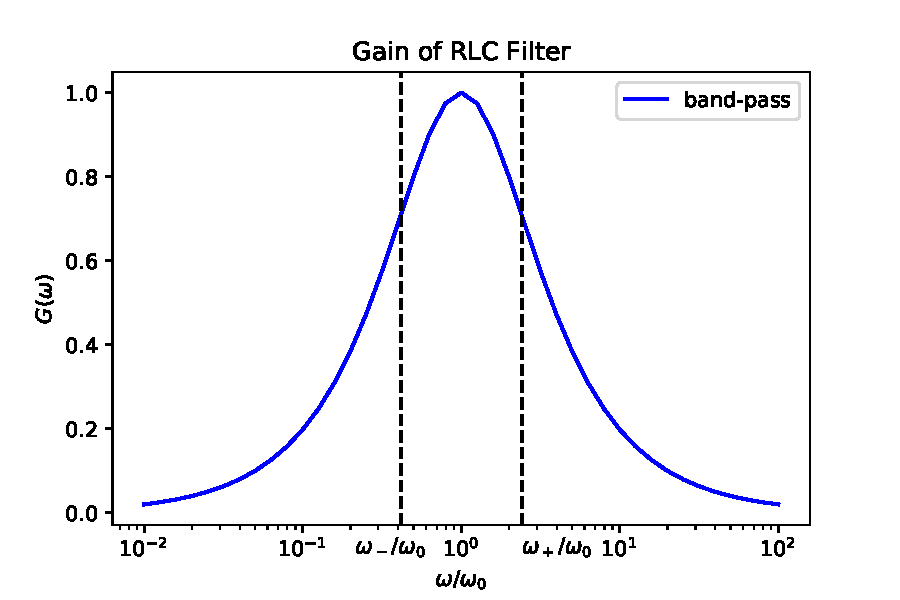
\includegraphics[height=0.3\textheight]{figs/rlcgain.pdf} \\
\caption{ The gain of the $RLC$ filter from Fig.~\ref{fig:rlcfilter}.}
\label{fig:rlcgain}
\end{center}
\end{figure}


Let's define two points $\omega_+$ and $\omega_-$ as the two
frequencies, one above and one below $\omega_0$, at which the gain
drops below $1/\sqrt{2}$.  These are the two $-3~\rm dB$ points which
define the bandwidth of the system.  The quality of the
resonance is defined by the ratio of resonant frequency to this bandwidth:

\begin{displaymath}
Q = \frac{\omega_0}{\omega_+ - \omega_-} = \frac{f_0}{f_+-f_-}
\end{displaymath}

The quality factor describes how under-damped a resonator is: the higher the Q factor the less damping there is. In $RLC$ circuit damping is caused by the loss of energy in resistive components. Quality factor can also be described as 
\begin{displaymath}
Q \propto \frac{\mbox{Maximum Energy Stored}}{\mbox{Energy Loss per cycle at resonance }}
\end{displaymath}
For the $RLC$ filter from Fig.~\ref{fig:rlcfilter}, $Q=\omega_0 \tau$. For a fixed values of $L$ and $C$, the quality factor of this circuit increases with increasing $R$. In reality, there will always be some parasitic resistance parallel and in series to $C$ and $L$, and this will lower the quality factor of the circuit.

\section{Exercises}
\begin{enumerate}
\item Show that for a sinusoidal AC voltage $v_{\rm rms} = v_{\rm p} / \sqrt{2}$.
\item Derive the steady-state solution Equation~\ref{eqn:inductorss} and the general solution Equation~\ref{eqn:inductorgen} for the LR circuit of Fig.~\ref{fig:rl}.


\item Use the impedance formula for capacitors $Z=1/j \omega C $ plus the formulas for equivalent impedance of parallel and series impedances to derive the usual formulas for the equivalent capacitance  of two capacitors in parallel:
\begin{displaymath}
C_{\rm eq} = C_1 + C_2
\end{displaymath}
and in series:
\begin{displaymath}
\frac{1}{C_{\rm eq}} = \frac{1}{C_1} + \frac{1}{C_2}
\end{displaymath}

\item Use the impedance formula for inductors $Z=j \omega L $ plus the formulas for equivalent impedance of parallel and series impedances to derive the usual formulas for the equivalent capacitance  of two inductors in parallel:
\begin{displaymath}
\frac{1}{L_{\rm eq}} = \frac{1}{L_1} + \frac{1}{L_2}
\end{displaymath}
and in series:
\begin{displaymath}
L_{\rm eq} = L_1 + L_2
\end{displaymath}
\item On the complex plane, draw three vectors for the impedance of an inductor, resistor, and capacitor and show that phase factors from Table~\ref{tbl:impedance} can be read directly from plot.
\item Show that you can construct a low-pass and high-pass filter using an inductor and resistor in series and determine the corner angular frequency $\omega_0$ in terms of the inductance $L$ and the resistance $R$.  Note that such filters are rarely used, because real inductors are expensive and generally have more non-ideal characteristics.
\begin{figure}[htbp]
\begin{center}
\begin{circuitikz}[line width=1pt]
\draw (0,0) to[sinusoidal voltage source,bipoles/length=1.5cm] ++(0,3.0) 
to[R,-*,l_=$R$] ++(2.0,0) coordinate(X) to[short,*-*] ++(1.5,0) coordinate(Y) to[short,-o] ++(1.0,0) node[right]{$\tilde{v}_{\rm out}$};
\draw (0.0,2.25) node[left]{$\tilde{v}_{\rm in}$};
\draw (X) to[C,-*,l=$C$] ++(0,-3.0)  to[short,-*] ++(-2.0,0) node[ground,yscale=2.0]{};
\draw (Y) to[L,-*,l=$L$] ++(0,-3.0)  coordinate(X) to[short,-*] ++(-1.5,0);
%\draw (X) to[short,-o] ++(1.0,0) node[right]{A};
\end{circuitikz}  
\caption{A function generator driving a resistor.}
\label{fig:rlccircuit}
\end{center}
\end{figure}
\item Consider the RLC filter of Fig.~\ref{fig:rlccircuit}.  Derive the transfer function for the circuit and find the resonant angular frequency $\omega_0$ for which the gain is 1.
\end{enumerate}



